\section{Air hockey as an MDP}
\label{sec:air_hockey_mdp}

This section describes how the Air hockey environment was modeled as an MDP by defining the state-action space and the employed reward functions.

\subsection{State space}

The observations provided by the original environment were slightly modified. Indeed the angular position $\theta$ and velocity $\dot{\theta}$ of the puck was discarded as well
as the z-axis element of the puck's position ${p}_{puck}$ and velocity ${\dot{p}}_{puck}$. The end-effector's position ${p}_{ee}$ and velocity
${\dot{p}}_{ee}$ were computed using the forward kynematics of the robot:

\begin{equation*}
    \begin{aligned}
        &{p}_{ee} = FK({q}) \\
        &{\dot{p}}_{ee} = {J}({q}){\dot{q}}
    \end{aligned}
\end{equation*}

where $q = \{q_i | i \in 1, \dots, 7, q^{\min}_i \le q_i \le q^{\max}_i \}$ fully represents the joint angles of the robot, $FK$ is the forward kynematics function and ${J}$ is the geometric Jacobian matrix of the forward kynematics function. Also the z-axis component of the position and velocity of the end-effector
were discarded. The resulting state space is given by
        
\begin{equation*}
    {s} = \begin{bmatrix}
            {p}_{puck} & {\dot{p}}_{puck} & {q} & {\dot{q}} & {p}_{ee} & {\dot{p}}_{ee}
        \end{bmatrix}
\end{equation*}


with $s \in \mathbb{R}^{22}$ for the 7 DoF robot and $s \in \mathbb{R}^{17}$ for the 3 DoF robot.
Finally, the state space was scaled between -1 and 1:

\begin{equation*}
    {s}_{scaled} = \frac{2\left(s - s_{low}\right)}{s_{high} - s_{low}} - 1
\end{equation*}

where $s_{low} \le s \,\forall s$ and $s_{high} \ge s\,\forall s$.

% Because of the noise added to the environment during the evaluation a Kalman Filter \cite{kalman_filter} was used on the puck's position.
% The noisy observations of joint positions and velocities were ignored and the reference joint positions and velocities given to the underlying controller at the previous step were used instead.

\subsection{Action space}
\label{subseq:action_space}
Two different approaches were used for modeling the action space.

\textit{Task space control}:
A high-level control setting where the agent controls the end-effector's position. This is achievable using the inverse kynematics of the robot
to find a configuration of the robot that places the end-effector in the wanted position.

\begin{equation*}
    \begin{aligned}
        &\bar{q}_t = IK(\bar{p}_{ee,t}) \\
        &\dot{\bar{q}}_t = \frac{\bar{q}_t - q_{t-1}}{\delta t}
    \end{aligned}
\end{equation*}

where $\bar{q}_t$ is the desired joint configuration computed using inverse kynematics from the desired end-effector's potision $p_{ee,t}$ at time $t$ and
$\dot{\bar{q}}_t$ is the desired joint velocity computed using finite differences.

The computed joint velocities were next optimized using \textit{weighted null space optimization}, defined in \ref{sec:baseline}, that takes into account the joint velocity limits.

\textit{Joint space control}:
The agent directly controls the joint accelerations $\ddot{q}$. This control variable is then converted to joint position and velocities using ATACOM \cite{Atacom} and submitted as a reference variable
to the underlying controller. The ATACOM transformation produces a command [joint\_positions, joint\_velocities] that reduces greatly the number of violated constraints excluding the joint velocity constraint.
Reducing the joint acceleration limits solved the joint velocity constraints problem. The action space too was scaled between -1 and 1.

\subsection{Reward function}
\label{subseq:reward}
The designed reward is task-dependent, given that a policy is trained for each task. It is also shaped as the success reward of each task is very sparse.
Generally the reward function introduces a penalty for each violated constraint proportional to its penalty points:

\begin{equation}
    r(s,a) = r_t(s,a) + r_c(s,a),
\end{equation}

where $r_t(s,a)$ is the task-dependent reward and $r_c(s,a)$ is the penalty for violating the constraints.


Additional tasks other than the ones specified in \ref{sec:organization} were designed for learning behaviors useful for a complete game. A \textit{return home} task in which the robot needs to achieve a certain configuration and remain still,
and a \textit{counter-attack} similar to the \textit{defend} task but gives the robot the possibility to score a goal while defending from the incoming puck.

The reward function $r_t(s,a)$ for each task is now described:

\textbf{Defend and counter-attack}: 
Two agents for the defend and counter-attack tasks. In these
tasks the episode starts with the puck moving towards our goal. In both cases, the agent receives a
high penalty (-100) when the puck breaches our goal. When the agent successfully interacts with the
puck, a reward (+10) is granted, coupled with reward proportional to the norm of the puck's velocity,
with a negative sign while defending and positive sign while counter-attacking. This incentivizes the
agent to interact with the puck and lower its velocity while also protecting the goal in the defend task,
while pushing back the puck in the counter-attack. Moreover, in the counter-attack, the agent can also
score in the opponent's goal, for which he receiver an additional large bonus of 1000.

\begin{equation*}
    r = \left\{
        \begin{aligned}
            1000 \quad &if \text{ scored} \\
            10 + A \cdot \Vert \dot{p}_{puck} \Vert \quad &if \text{ interacted with puck} \\
            -100 \quad &if \text{ opponent scored a goal}
        \end{aligned}
    \right.
\end{equation*}

where $A$ is a constant term with positive sign in the counter-attac task, negative in the defend task.

\textbf{Hit}:
The reward function of the hit task is based on the construction of a triangle with the opponent's area and the puck as vertices (Figure \ref{fig:triangle_reward}).
If the puck, after the hit, lies inside the triangle, a reward is assigned, proportional to the puck's velocity; if the puck is outside the triangle, a penalty is assigned.
The more the puck is outside the polygon, the bigger the penalty.

\begin{equation*}
    r_{\text{before hit}} = \left\{
        \begin{aligned}
            -\frac{\Vert p_{ee} - p_{puck} \Vert}{0.5 \, \text{table\_diag}} \quad &if \text{ no hit,} \\
            100 + 10\,\frac{\left(1 - \left(2\frac{\alpha}{\pi}\right)^2\right)\Vert \dot{p}_{ee} \Vert}{\text{max\_vel}} \quad &if \text{ hit the puck,} \\
            \frac{1}{1 - \gamma} \quad &if \text{ scored}
        \end{aligned}
    \right.
\end{equation*}

where \textit{table\_diag} is the diagonal of the table and \textit{max\_vel} is a constant equal to the maximum velocity observable in the environment,
while $\alpha = \arctantwo(p_{ee,y}, p_{ee,x})$.

If the agent hits the puck, it receives an instantaneous reward and, after that, the triangle approach is applied.

\begin{equation*}
    r_{\text{after hit}} = \left\{
        \begin{aligned}
            10 + \Vert \dot{p}_{puck} \Vert \quad  &if \text{ puck inside triangle}, \\
            -\text{diff\_angle} \quad              &if \text{ otherwise} 
        \end{aligned}
    \right.
    \end{equation*}


\begin{equation*}
    \text{diff\_angle} = \arctantwo\left(\dot{p}_{puck,y},\dot{p}_{puck,x}, \right) - \text{angle\_border}
\end{equation*},

where angle\_border is the angle between the puck velocity vector and the closest triangle border.

\begin{figure}[H]
    \centering
    \subfloat[Triangle computation at step $t$.]{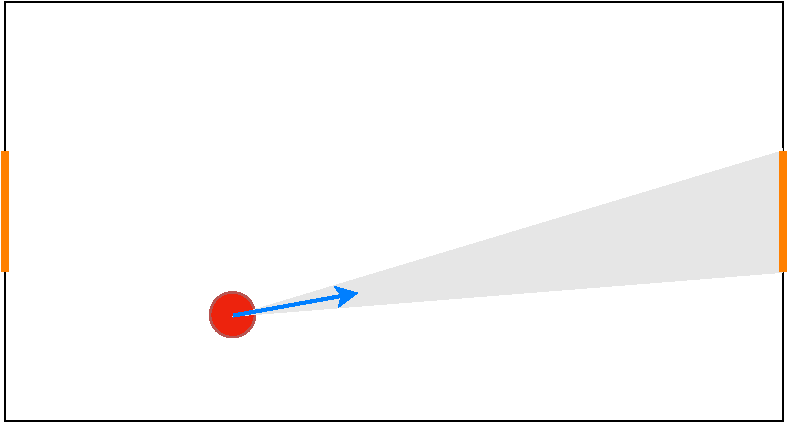
\includegraphics[width=0.35\linewidth]{Images/triangle_1.pdf}}
    \hskip1ex
    \subfloat[Puck moving and reward assignment at step $t+1$.]{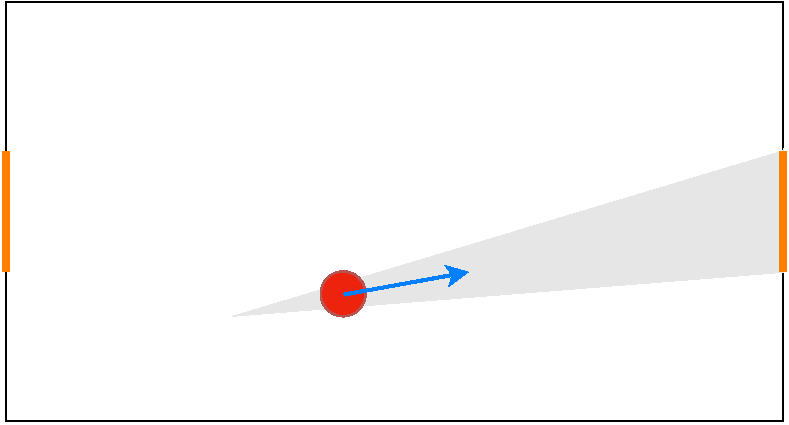
\includegraphics[width=0.35\linewidth]{Images/triangle_2.pdf}}

    \caption{Triangle construction for assigning reward after the mallet hit the puck.}
    \label{fig:triangle_reward}
\end{figure}

\textbf{Prepare}:
The reward function for the prepare task is a sparse reward given at the last step with a high reward (1000) if the task is successful, otherwise -100.

\textbf{Return home}: At each step of the training process, the agent incurs a penalty based on the distance to the \textit{home configuration}
\begin{equation*}
    r = - \Vert q - q_{home} \Vert
\end{equation*}

where $q_{home}$ is the initial position of the robot before a game starts or after a reset. For this task, the robot was initialized to a configuration
drawn from the distribution of terminal states of the other tasks.
This distribution is necessary for creating experiments with different initial positions, ensuring that the agent can learn to reach $q_{home}$ independently of its starting position.




